\section{Baseline Comparison}
\label{sec:baseline-comparison}

For the purpose of evaluating GaitNet's performance, a baseline
method is established using a single leg motion planner. This planner
operates as is described in \cite{bratta_contactnet_2024}, where in
place of ContactNet, we directly use the footstep evaluation  network
described in \autoref{label}

\autoref{fig:data-terrain-evaluation-comparison} illustrates the
performance of GaitNet relative to the baseline method across a range
of terrain difficulties and commanded velocities. The results
indicate that GaitNet outperforms the baseline in most scenarios,
particularly on more challenging terrains and at higher commanded
speeds. This demonstrates the effectiveness of GaitNet in generating
robust gaits capable of adapting to varying conditions.

A closer examination of the graphs reveals that GaitNet maintains
strong performance when the commanded velocity is below 0.15\,m/s or
terrain difficulty is under 5\%. In contrast, ContactNet's
performance begins to degrade for commanded velocities above
0.05\,m/s and deteriorates further as terrain difficulty increases.
GaitNet's superior performance in these scenarios underscores the
benefits of its dynamic, acyclic gait generation capabilities.

\begin{figure}[H]
  \centering
  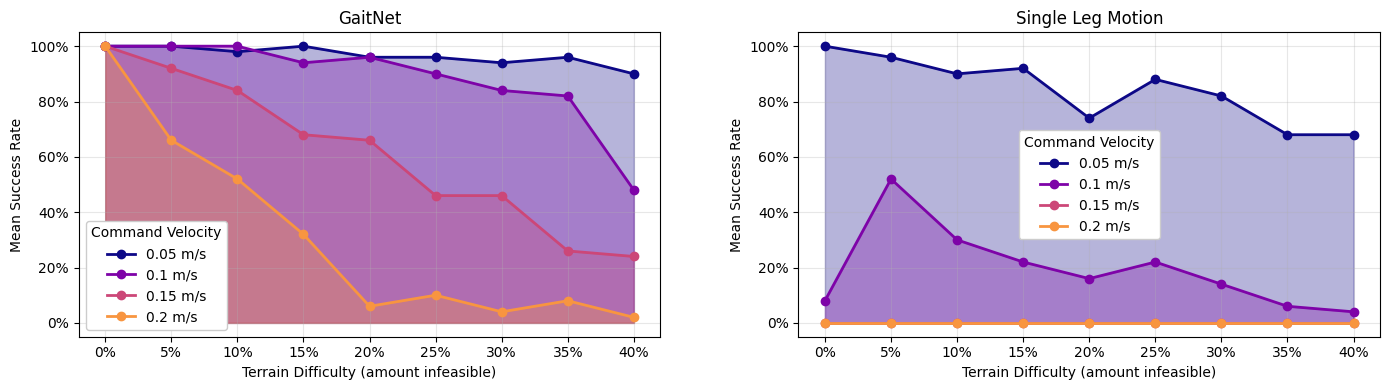
\includegraphics[width=\textwidth]{images/data/terrain-evaluation-comparison.png}
  \caption{Evaluation of GaitNet vs. single leg motion planner
    across various terrain difficulties and commanded velocities.
    Mean success rate measured as the percentage of 50 episodes
    which completed 20\,s without terminating, under the termination
  conditions described in \autoref{sec:appendix-termination-functions}.}
  \label{fig:data-terrain-evaluation-comparison}
\end{figure}
